\chapter{Practice Exam 1}
    Cyril the Circuit Analyst is examining the interaction of both AC and DC sources with a circuit.
    The circuit is drawn below. Pay careful attention to the arrows on the switches which show
    which are initially open, and which are initially closed. Assume that the capacitor is initially
    discharged at t = 0. All times are in seconds.
    \begin{figure}[H]
        \centering
        \begin{circuitikz}[american]
            \draw (0,0)
                to [current source, i=10mA] (0,2)
                to [switch, l=$\text{t=0s}$] (1,2)
                to [opening switch, l=$\text{t=1s}$] (3,2)
                to [switch, l=$\text{t=2s}$] (5,2)
                to [switch, l=$\text{t=5s}$] (7,2)
                to [inductor, l=100$\mu$F] (9,2)
                to [sinusoidal voltage source, v=$10\cos(\omega t)$] (9,0)
                to [short] (0,0);
            \draw (3,2)
                to [capacitor, l=50$\mu$F] (3,0) node[ground] {};
            \draw (5,2)
                to [resistor, l=400$\Omega$] (5,0);
        \end{circuitikz}
    \end{figure}
    \begin{enumerate}
        \item At t = 0, the first switch closes connecting the current source to the capacitor. Find the
        voltage on the capacitor at t = 1 second\\
        \textbf{Solution:}\\
        \begin{minipage}{0.4\linewidth}
            \begin{figure}[H]
                \centering
                \begin{circuitikz}[american]
                    \draw (0,0)
                        to [current source, i=10mA] (0,2)
                        to [short] (2,2)
                        to [capacitor, l=50$\mu$F] (2,0)
                        to [short] (0,0);
                \end{circuitikz}
            \end{figure}
        \end{minipage}
        \begin{minipage}{0.5\linewidth}
            \begin{flalign*}
                v(t) &= \frac{1}{C} \int^{t}_{0} i(\tau)\ d\tau + v(0)\\
                &= \frac{1}{50\times 10^{-6}} \int^{1}_{0} 10\times 10^{-3}\ d\tau + 0\\
                &= 200\text{V}
            \end{flalign*}
        \end{minipage}
        \item At t = 1, the second switch opens disconnecting the current source from the capacitor.
        Find the voltage on the capacitor at t = 2 seconds.\\
            \textbf{Solution:}\\
            The capacitor is not connected to any circuit elements. Therefore, the voltage across the
            capacitor will remain constant at 200V for $1 < t < 2$.
        \item At t = 2, the third switch closes connecting the capacitor to the resistor. Find the voltage
        on the capacitor at t = 2.1 seconds\\
            \textbf{Solution:}\\
            \begin{minipage}{0.4\linewidth}
                \begin{figure}[H]
                    \centering
                    \begin{circuitikz}[american]
                        \draw (0,0)
                            to [current source, i=10mA] (0,2)
                            to [short] (2,2)
                            to [capacitor, l=50$\mu$F] (2,0)
                            to [short] (0,0);
                    \end{circuitikz}
                \end{figure}
            \end{minipage}
            \begin{minipage}{0.5\linewidth}
                \begin{flalign*}
                    V(t) &= V(0)e^{-\frac{t}{RC}}\\
                    &= 200e^{-\frac{0.1}{400\times 50\times 10^{-6}}}\\
                    V(0.1) &= 200e^{-5\times 10^5 \times 10^{-1}} = 1.348\text{V}
                \end{flalign*}
            \end{minipage}
        \item At t = 5, the fourth switch closes connecting the AC source and inductor. The circuit
        reaches AC steady state at some $t >> 5$. Express the AC steady state voltage on the
        capacitor as a function of time using
        $\omega = 1000$ rad/s\\
            \textbf{Solution:}\\
            \begin{minipage}{0.5\linewidth}
                \begin{figure}[H]
                    \centering
                    \begin{circuitikz}[american]
                        \draw (0,0)
                            to [capacitor, l=50$\mu$F] (0,2)
                            to [short] (2,2)
                            to [inductor, l=10mH] (4,2)
                            to [sinusoidal voltage source, v=$10\cos(\omega t)$] (4,0)
                            to [short] (0,0);
                        \draw (2,2)
                            to [resistor, l=400$\Omega$] (2,0);
                    \end{circuitikz}
                \end{figure}
            \end{minipage}
            \begin{minipage}{0.4\linewidth}
                \begin{flalign*}
                    V_{\text{out}} &= \frac{Z_R || Z_C}{(Z_R || Z_C) + Z_L} V_{\text{in}} \tag{Voltage divider}\\
                    &= \frac{\frac{1}{j\omega C} || R}{\frac{1}{j\omega C} || R + j\omega L}V_{\text{in}}\\
                    &= \frac{\left(j\omega C + \frac{1}{R}\right)^{-1}}{\left(j\omega C + \frac{1}{R}\right)^{-1} + j\omega L} V_{\text{in}}\\
                    &= \frac{\left(\frac{1}{400} + j\times 10^3 \times 50^{-6} \right)^{-1}}{\left(\frac{1}{400} + j\times 10^3 \times 50^{-6} \right)^{-1} + j\times 10^3 \times 10^{-2}}\\
                    &= 19.95 - j0.998
                \end{flalign*}
            \end{minipage}
        \item Perform frequency response analysis for the circuit for t $>>$ 5 to calculate the gain in dB
        and phase in degrees for
        $\omega$ at 100 rad/s, 1000 rad/s and 10000 rad/s
        \begin{flalign*}
            H(\omega) &= \frac{V_{\text{out}}}{V_{\text{in}}} = \frac{Z_R || Z_C}{(Z_R || Z_C) + Z_L} \tag{Voltage divider}\\
            &= \frac{\frac{1}{j\omega C} || R}{\frac{1}{j\omega C} || R + j\omega L}\\
            &= \frac{\left(j\omega C + \frac{1}{R}\right)^{-1}}{\left(j\omega C + \frac{1}{R}\right)^{-1} + j\omega L}\\
            &= \frac{\left(\frac{1}{400} + j\omega \times 50\times 10^{-6} \right)^{-1}}{\left(\frac{1}{400} + j\omega \times 50\times 10^{-6} \right)^{-1} + j\omega \times 10^{-2}}\\
        \end{flalign*}
        \begin{figure}[H]
            \centering
            \begin{tabular}{ccc}
                $\boldsymbol{\omega}$ & \textbf{Gain (dB)} & \textbf{Phase (degrees)}\\
                \toprule
                100 & 0.435 & -0.144\\
                1000 & 5.998 & -2.86\\
                10000 & -33.804 & -179.71\\
            \end{tabular}
        \end{figure}
        \item Plot the response calculated in part (3) in a Bode plot\\
            \textbf{Solution:}\\
            \begin{figure}[H]
                \centering
                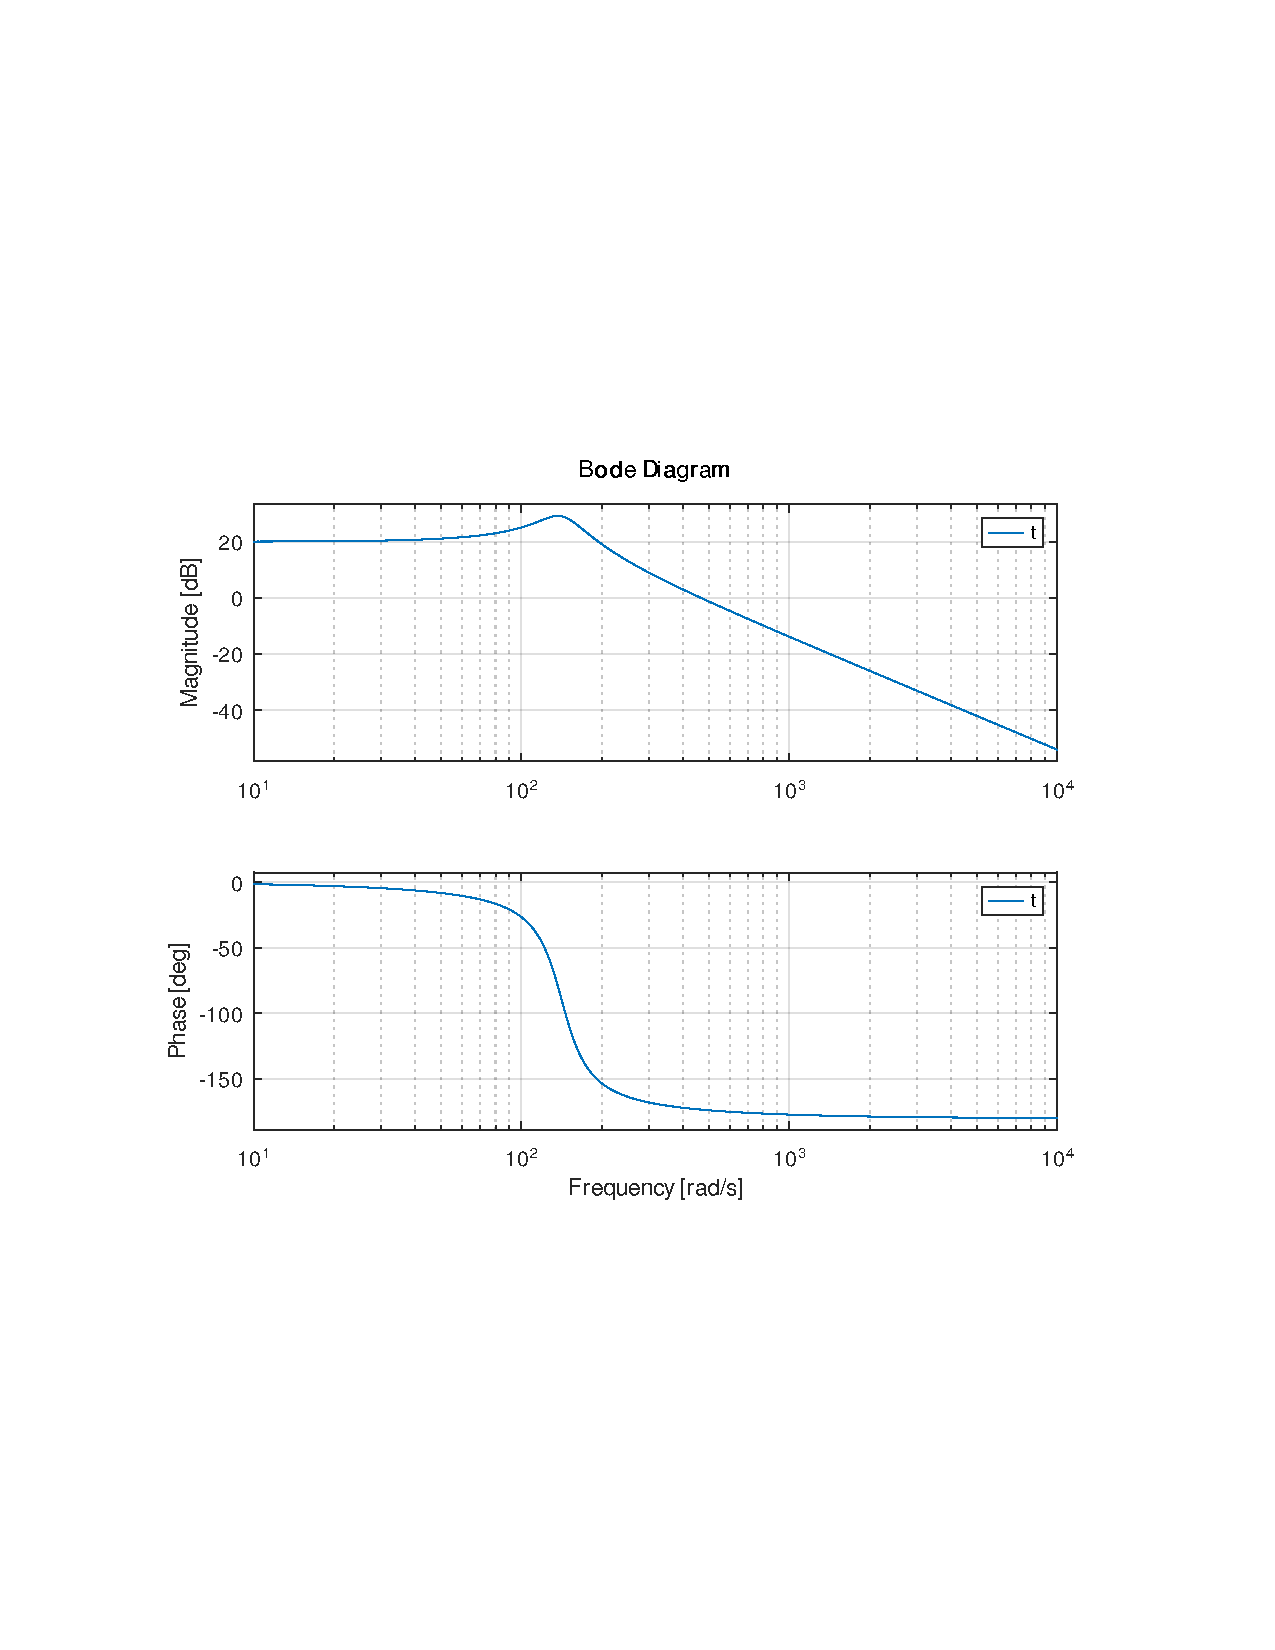
\includegraphics[width=0.8\linewidth,trim={0 7.5cm 0 7.5cm},clip]{figures/bodeplot.pdf}
            \end{figure}
    \end{enumerate}5